\section{Experiments}

\subsection{MONK's results}

\subsubsection{Architecture and hyper-parameters}
We have used a fully connected NN with layers of size 17-15-2, with a \texttt{tanh} activation function in the hidden layer, and a \texttt{softmax} for the output layer.

We chose \texttt{crossEntropy} as the loss function, i.e. if the output of the NN was $y=(y_1,y_2)$ and the label was $\hat y=(\hat y_1,\hat y_2)$, then $$L(y,\hat y)=-\hat y_1\log y_1-\hat y_2\log y_2$$

We used mini-batch gradient descent with $\texttt{batch\_size}=10$ and momentum with parameter $\beta$.

We also used L2 regularization with parameter $\lambda$.

Our choice of hyper-parameters is shown in \cref{fig:hyper} below, along with the performance.

\begin{figure}[h]
    \begin{tabular}{|l|c|c|c|c|c|}
        \hline 
        Task & $\eta$ & $\lambda$ & $\beta$ & Loss (train/valid) & Accuracy (train/test) \\ \hline
        MONK 1 & 0.1 & 0.003 & 0.8 & 0.0466/0.0552  & 100\%/100\% \\ \hline
        MONK 2 & 0.1 & 0.003 & 0.8 & 0.0531/0.0896 & 100\%/100\% \\ \hline
        MONK 3 (reg) & 0.01 & 0.02 & 0.9 & 0.2116/0.4599 & 94.2\%/97.2\% \\ \hline
        MONK 3 (non reg) & 0.1 & 0.0001 & 0.9 & 0.0052/0.7687 & 100\%/93.9\% \\ \hline
    \end{tabular}
    \caption{Performance results on MONK dataset}
    \label{fig:hyper}
\end{figure}


\subsubsection{Learning curves}

Now we show the learning curves of the three MONK tasks, plotting loss and accuracy over the training set and the validation set.

\begin{figure}
    \centering
    \subfloat[MONK 1]{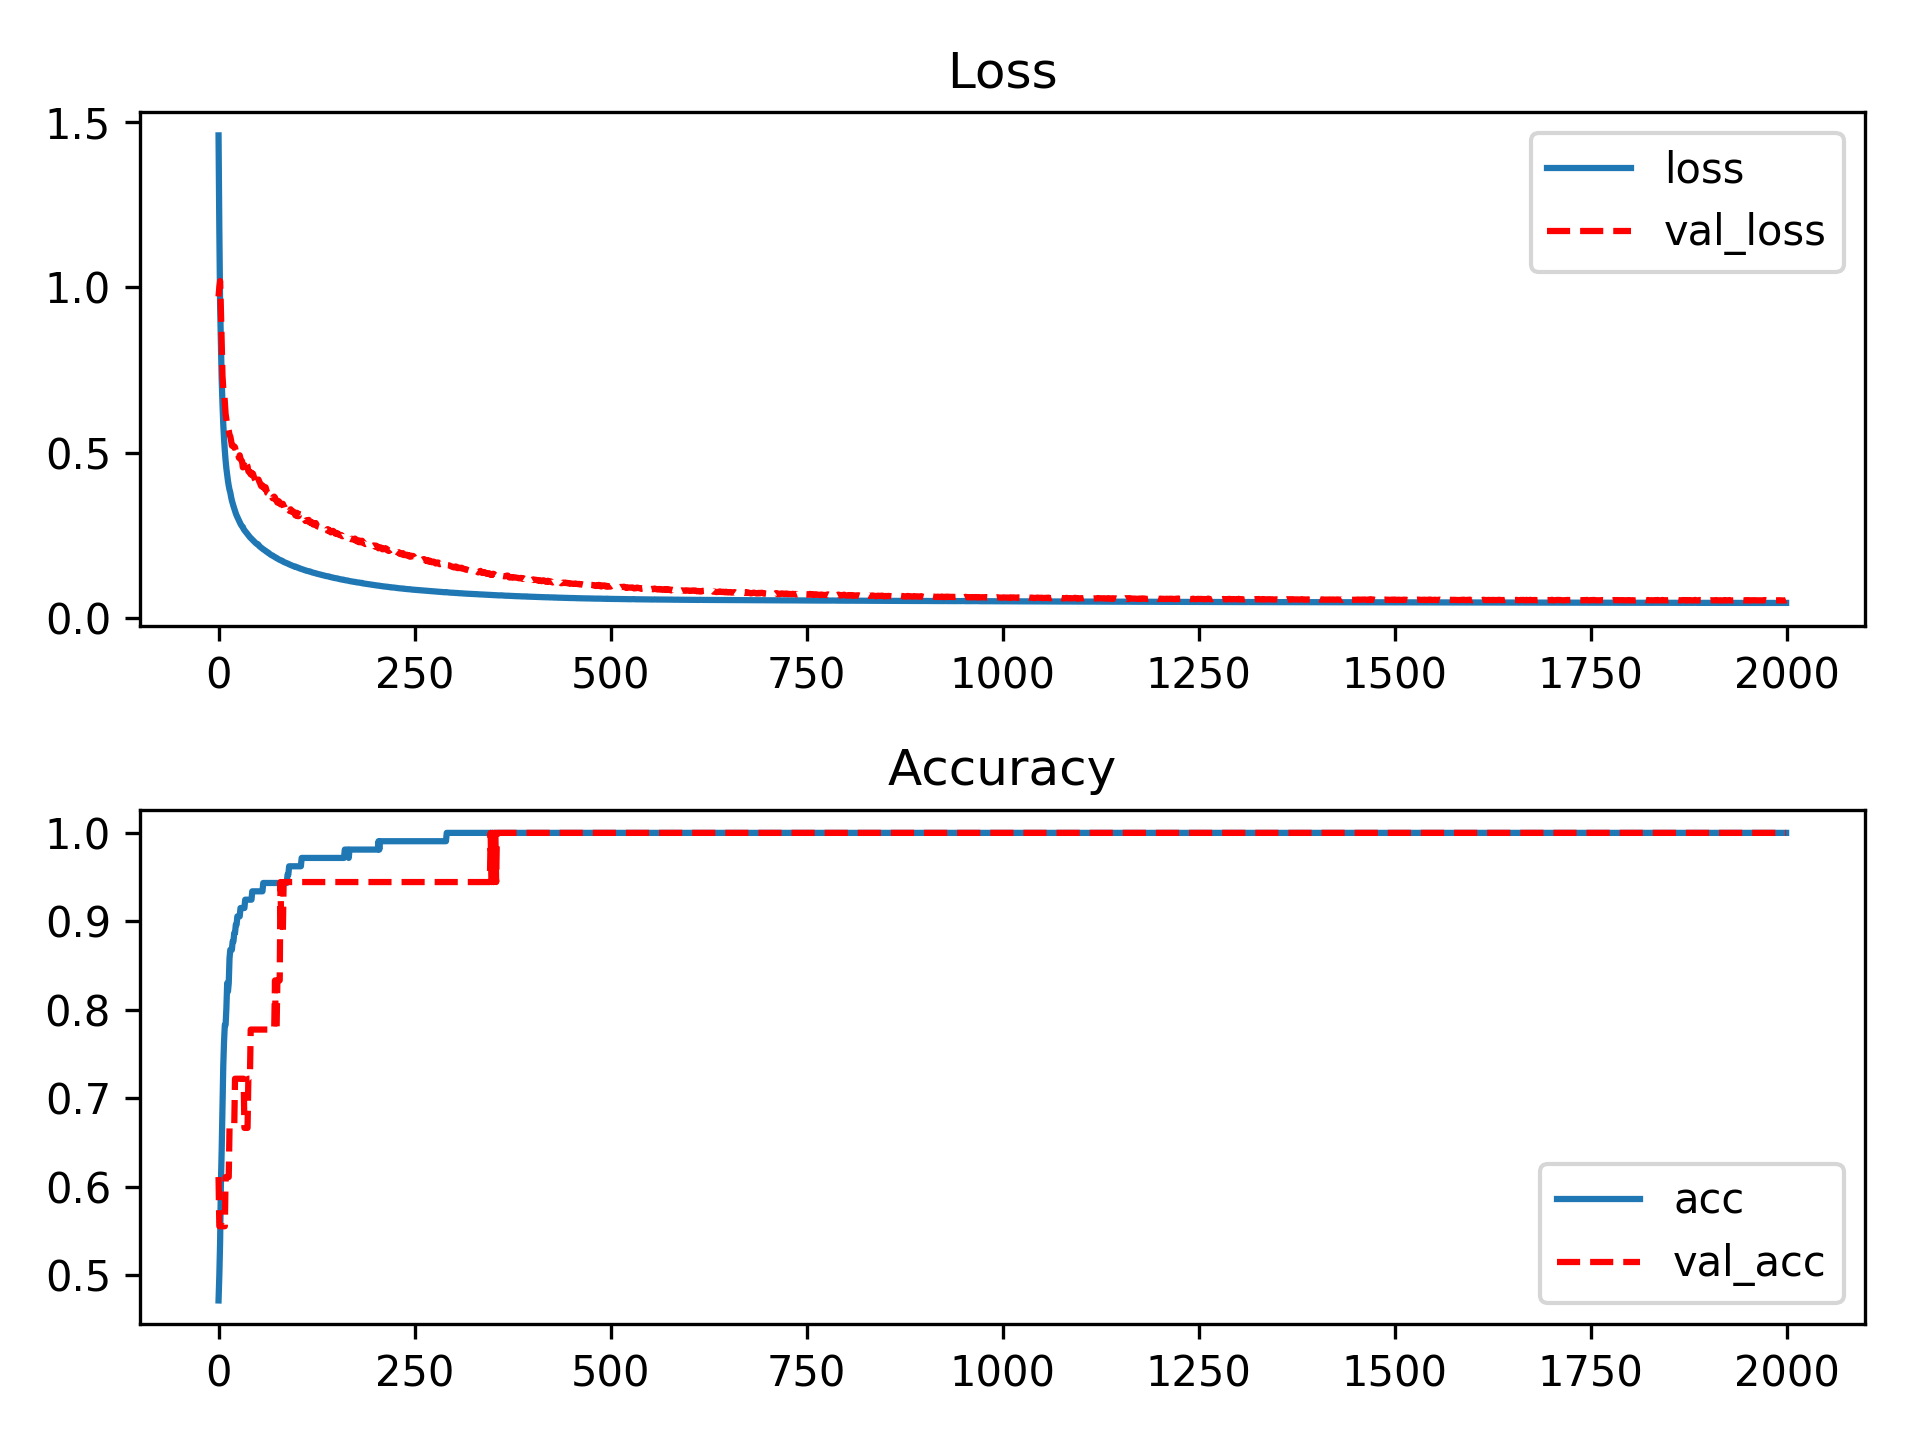
\includegraphics[width=0.5\textwidth]{monks1}}
    \subfloat[MONK 2]{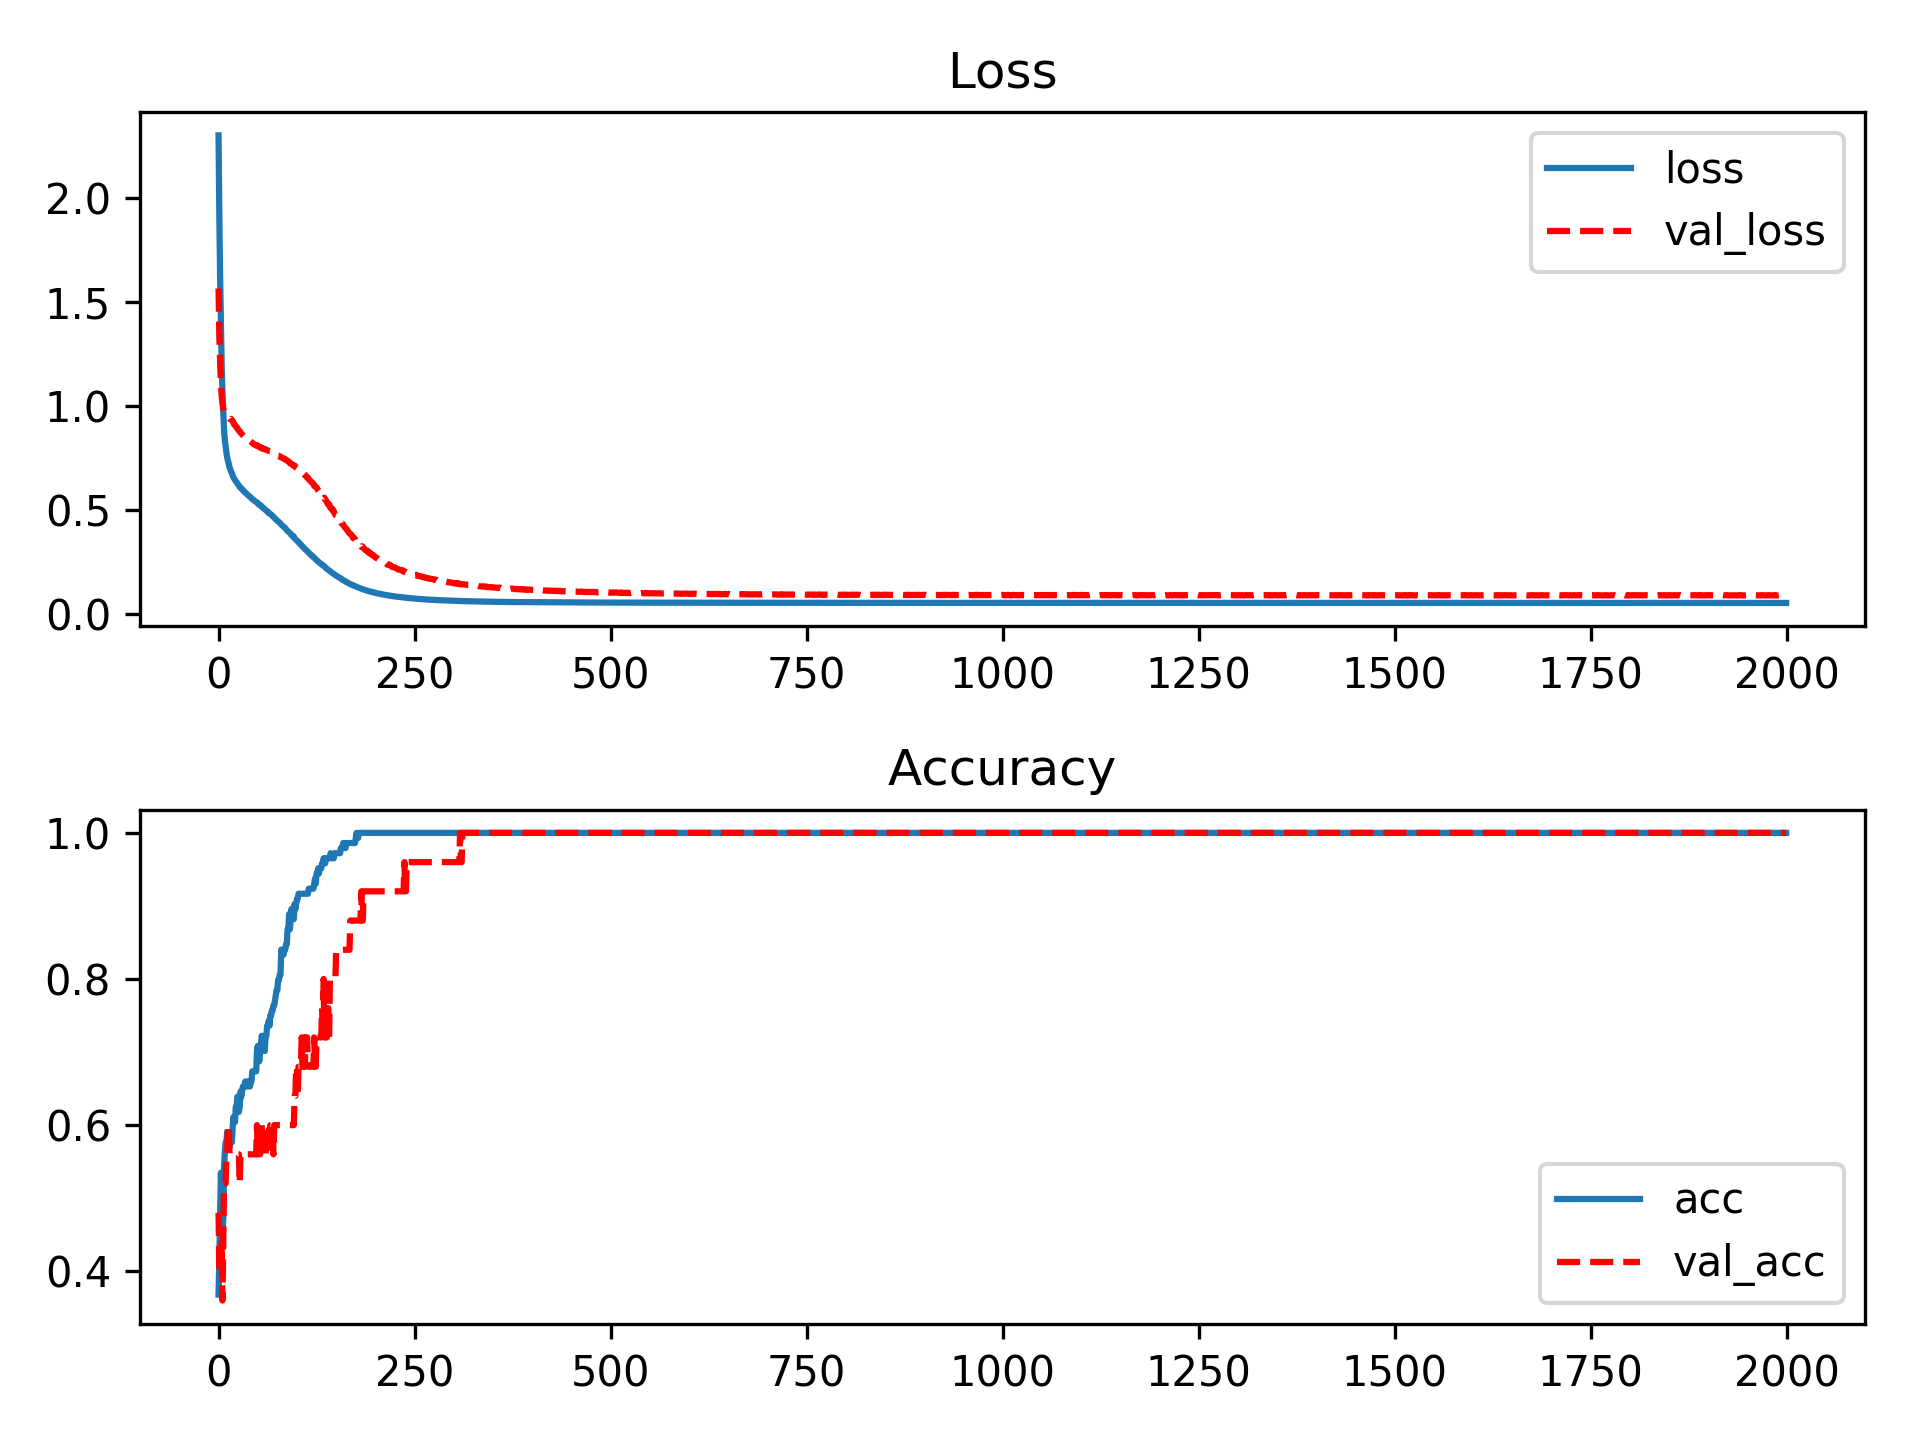
\includegraphics[width=0.5\textwidth]{monks2}}
    \caption{Learning curves on MONK 1 \& 2}
    \label{fig:monk12}
\end{figure}

\begin{figure}
    \centering    \subfloat[regularized\label{fig:monk3}]{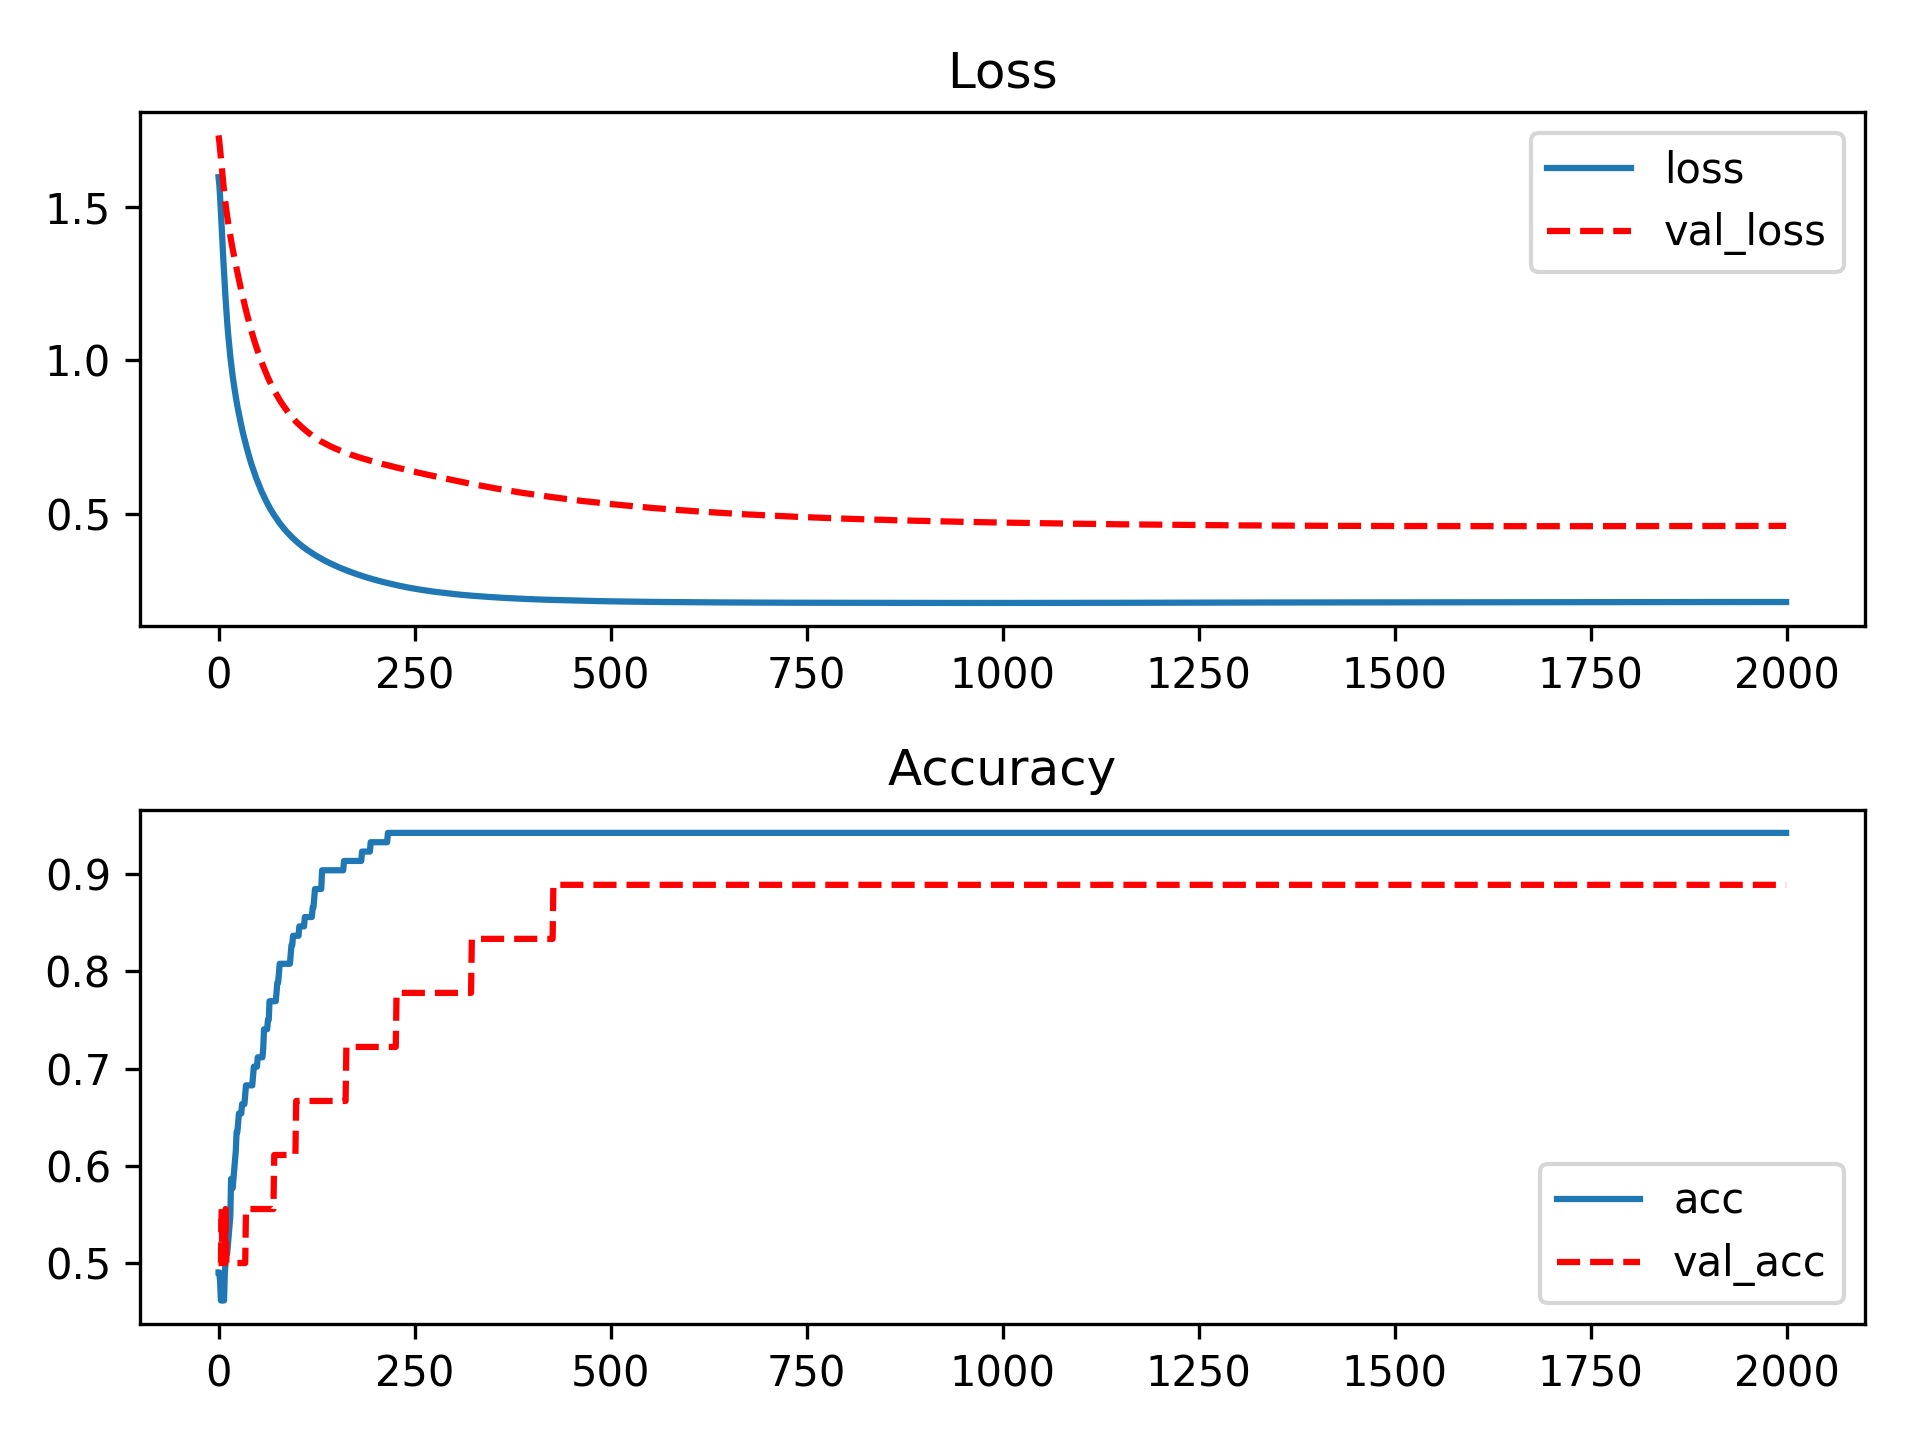
\includegraphics[width=0.5\textwidth]{monks3}}
    \subfloat[not regularized\label{fig:monk3-nr}]{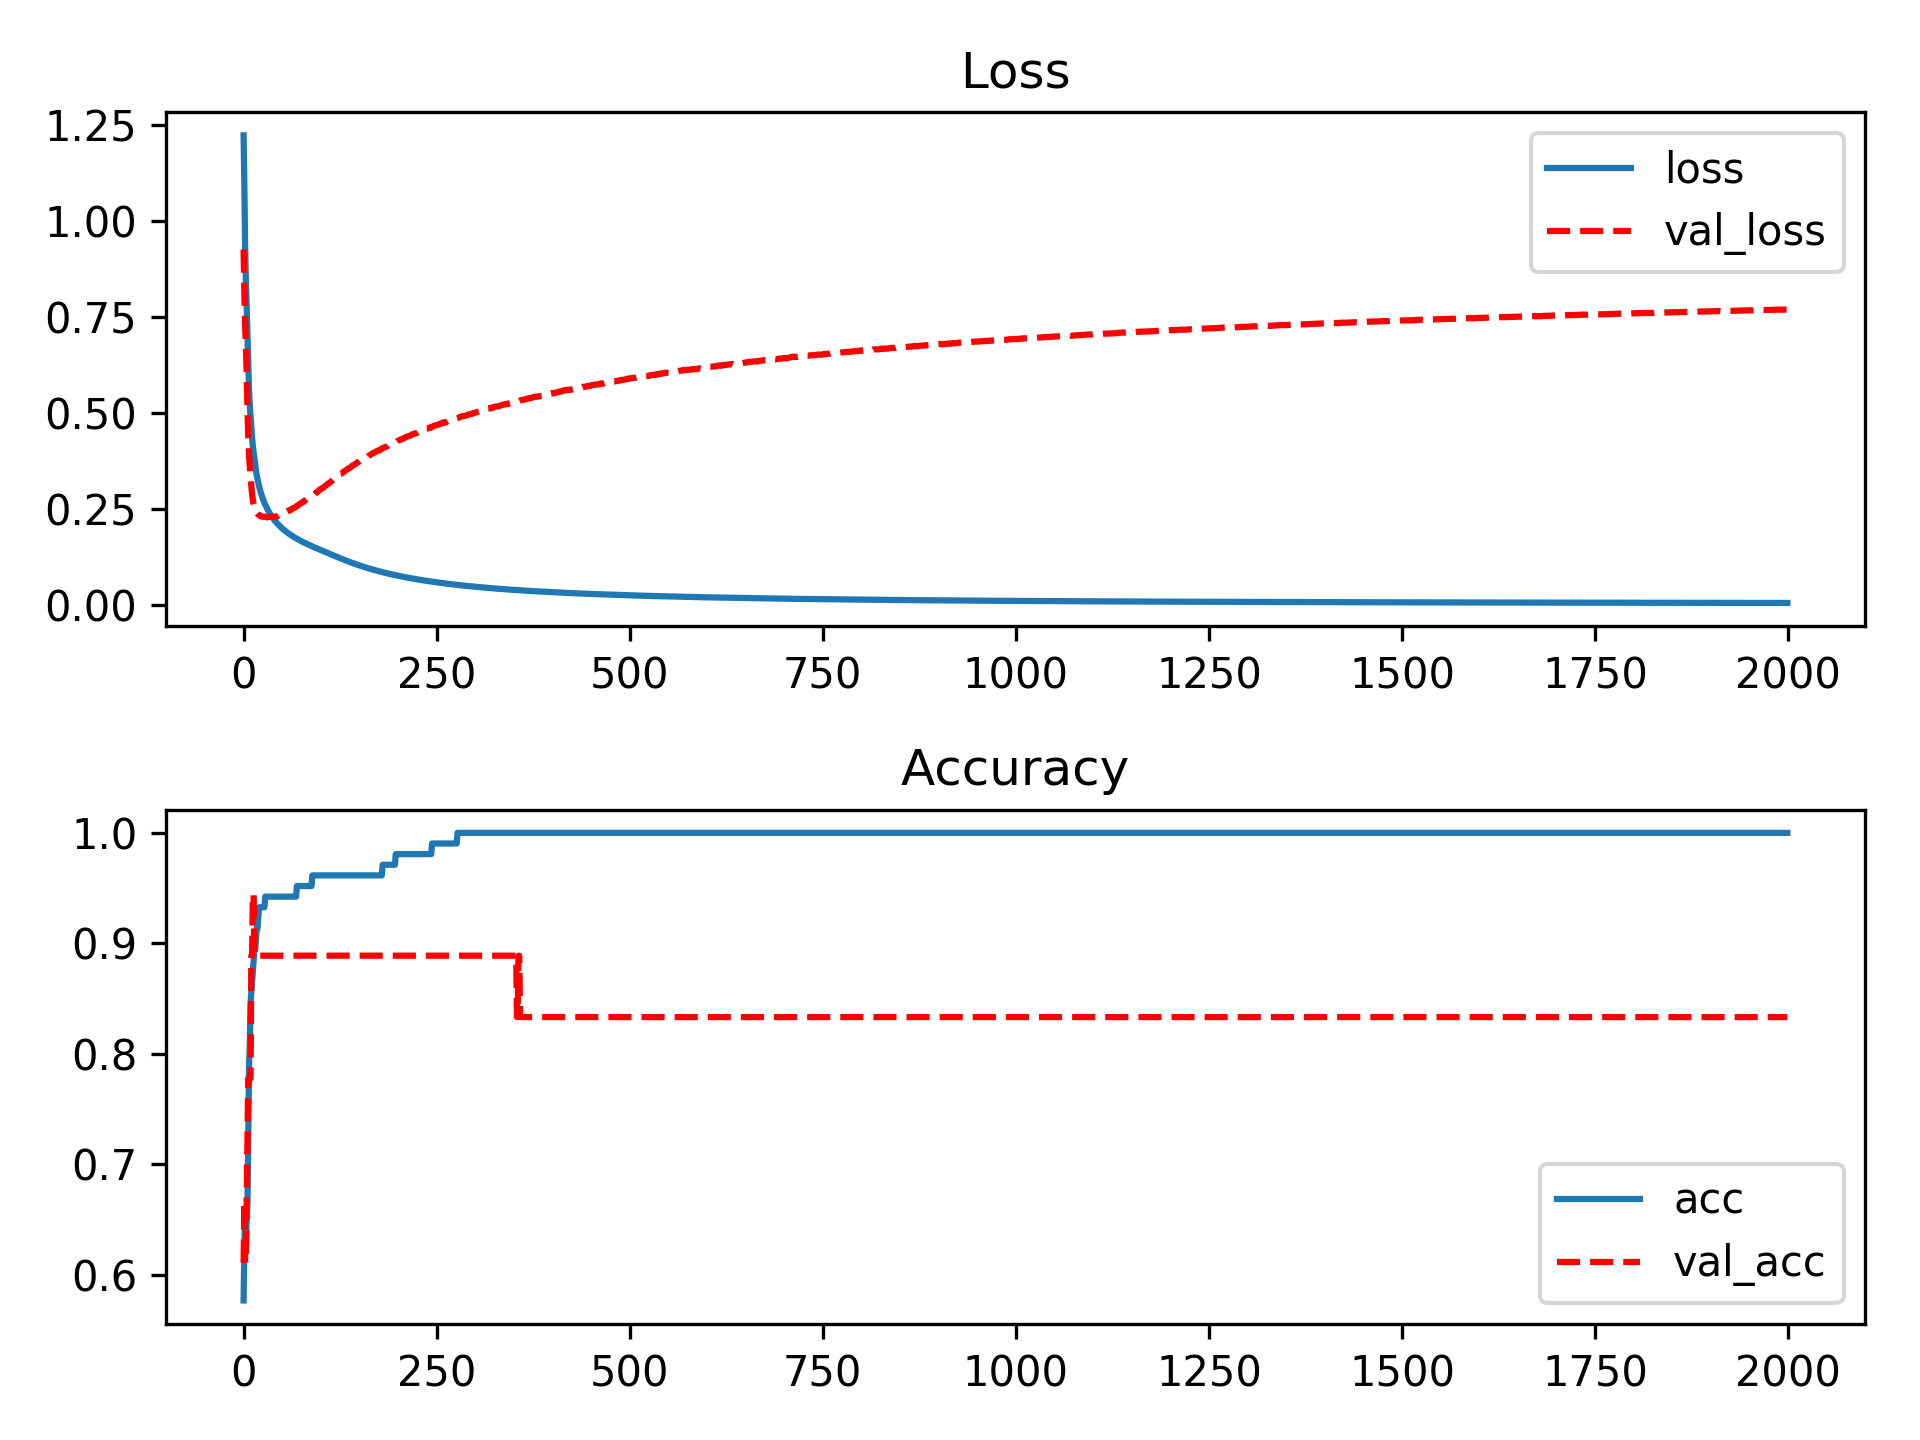
\includegraphics[width=0.5\textwidth]{monks3-nr}}
    \caption{Learning curves for MONK 3}
\end{figure}

We notice that the training loss of MONK 3 (\cref{fig:monk3}) is quite high: this is because the training set has some noise and hence we are keeping a quite strong regularization.
If instead we remove the regularization, then it overfits as shown in \cref{fig:monk3-nr}

\clearpage

\subsection{CUP results}

The first thing we did was to take 100 random data-points from the training set and put them in a separate file for internal testing. So we had 916 data-points for the actual training and validation.

For every training instance we randomly split the internal training set at random for 75\% actual training and 25\% validation. We always used mini-batch gradient descent with $\texttt{batch\_size}=32$.


\subsubsection{Preliminary trials}

We first tried to see if we needed a deep NN, but increasing the number of layers didn't yield significant improvements.

Then we chose to use MEE as the loss function instead of MSE, because it was the metric we actually strove to minimize.

So we wanted a model with layers 10-H-2 for some $H\in\{ 10, 20, 50 \}$, and an activation function in the hidden layer among \texttt{tanh}, \texttt{sigmoid}, \texttt{reLU} and \texttt{softMax}.

Then we had also to tune the hyper-parameters $\eta,\lambda,\beta$ so we performed a grid search on these 5 parameters, distributing the load among many machines.

\subsubsection{Grid search}

For each choice of an activation function and a number of hidden neurons $H$ we made a different machine run a grid search among these values:
\begin{itemize}
    \item $\eta\in\{ 0.1, 0.05, 0.01, 0.005, 0.001 \}$
    \item $\lambda\in\{ 0.005, 0.001, 0.0005, 0.0001 \}$
    \item $\beta\in\{ 0, 0.95 \}$
\end{itemize}

Our best results were achieved employing the \texttt{sigmoid} activation and $H=20$, on which we had the results shown below in \cref{fig:gridSearch}.

\begin{figure}[h]
    \centering
    \begin{tabular}{|c||c|c|c|c|c|}
            \hline
              $\lambda \backslash \eta$ & $0.1$ & $0.05$ & $0.01$ & $0.005$ & $0.001$\\ \hline\hline
             $0.005$ & 1.461 & 1.493 & 1.465 & 1.461 & 1.728 \\ \hline
             $0.001$ & 1.177 & 1.226 & 1.276 & 1.349 & 1.699 \\ \hline
             $0.0005$ & 1.193 & 1.175 & 1.249 & 1.317 & 1.668 \\ \hline
             $0.0001$ & 1.220 & 1.224 & 1.238 & 1.306 & 1.668 \\ \hline
    \end{tabular}
    \caption{Values of MEE for $H=20$, \texttt{sigmoid} and $\beta=0$}
    \label{fig:gridSearch}
\end{figure}

We run this computationally heavy grid search on multiple machines in a single night: for each choice of hyper-parameters we run the training for 2000 epochs for 10 trials, and then averaged the MEE score on the validation set.

\subsubsection{Chosen models}

As a result of the grid search our fist model had a topology of 10-20-2 with \texttt{sigmoid} activation, and we trained it for 2000 epochs with $\eta=0.1,\lambda=0.001,\beta=0$. Let's call this \emph{network of type A}.

We achieved an average MEE of $1.119$ on our blind test, taken as an average of 10 different trainings of type A networks (to avoid the bias due to the random weight initialization). We can see the learning curve of one of them in \cref{fig:typeA} below.

\begin{figure}[h]
    \centering
    \subfloat[Type A\label{fig:typeA}]{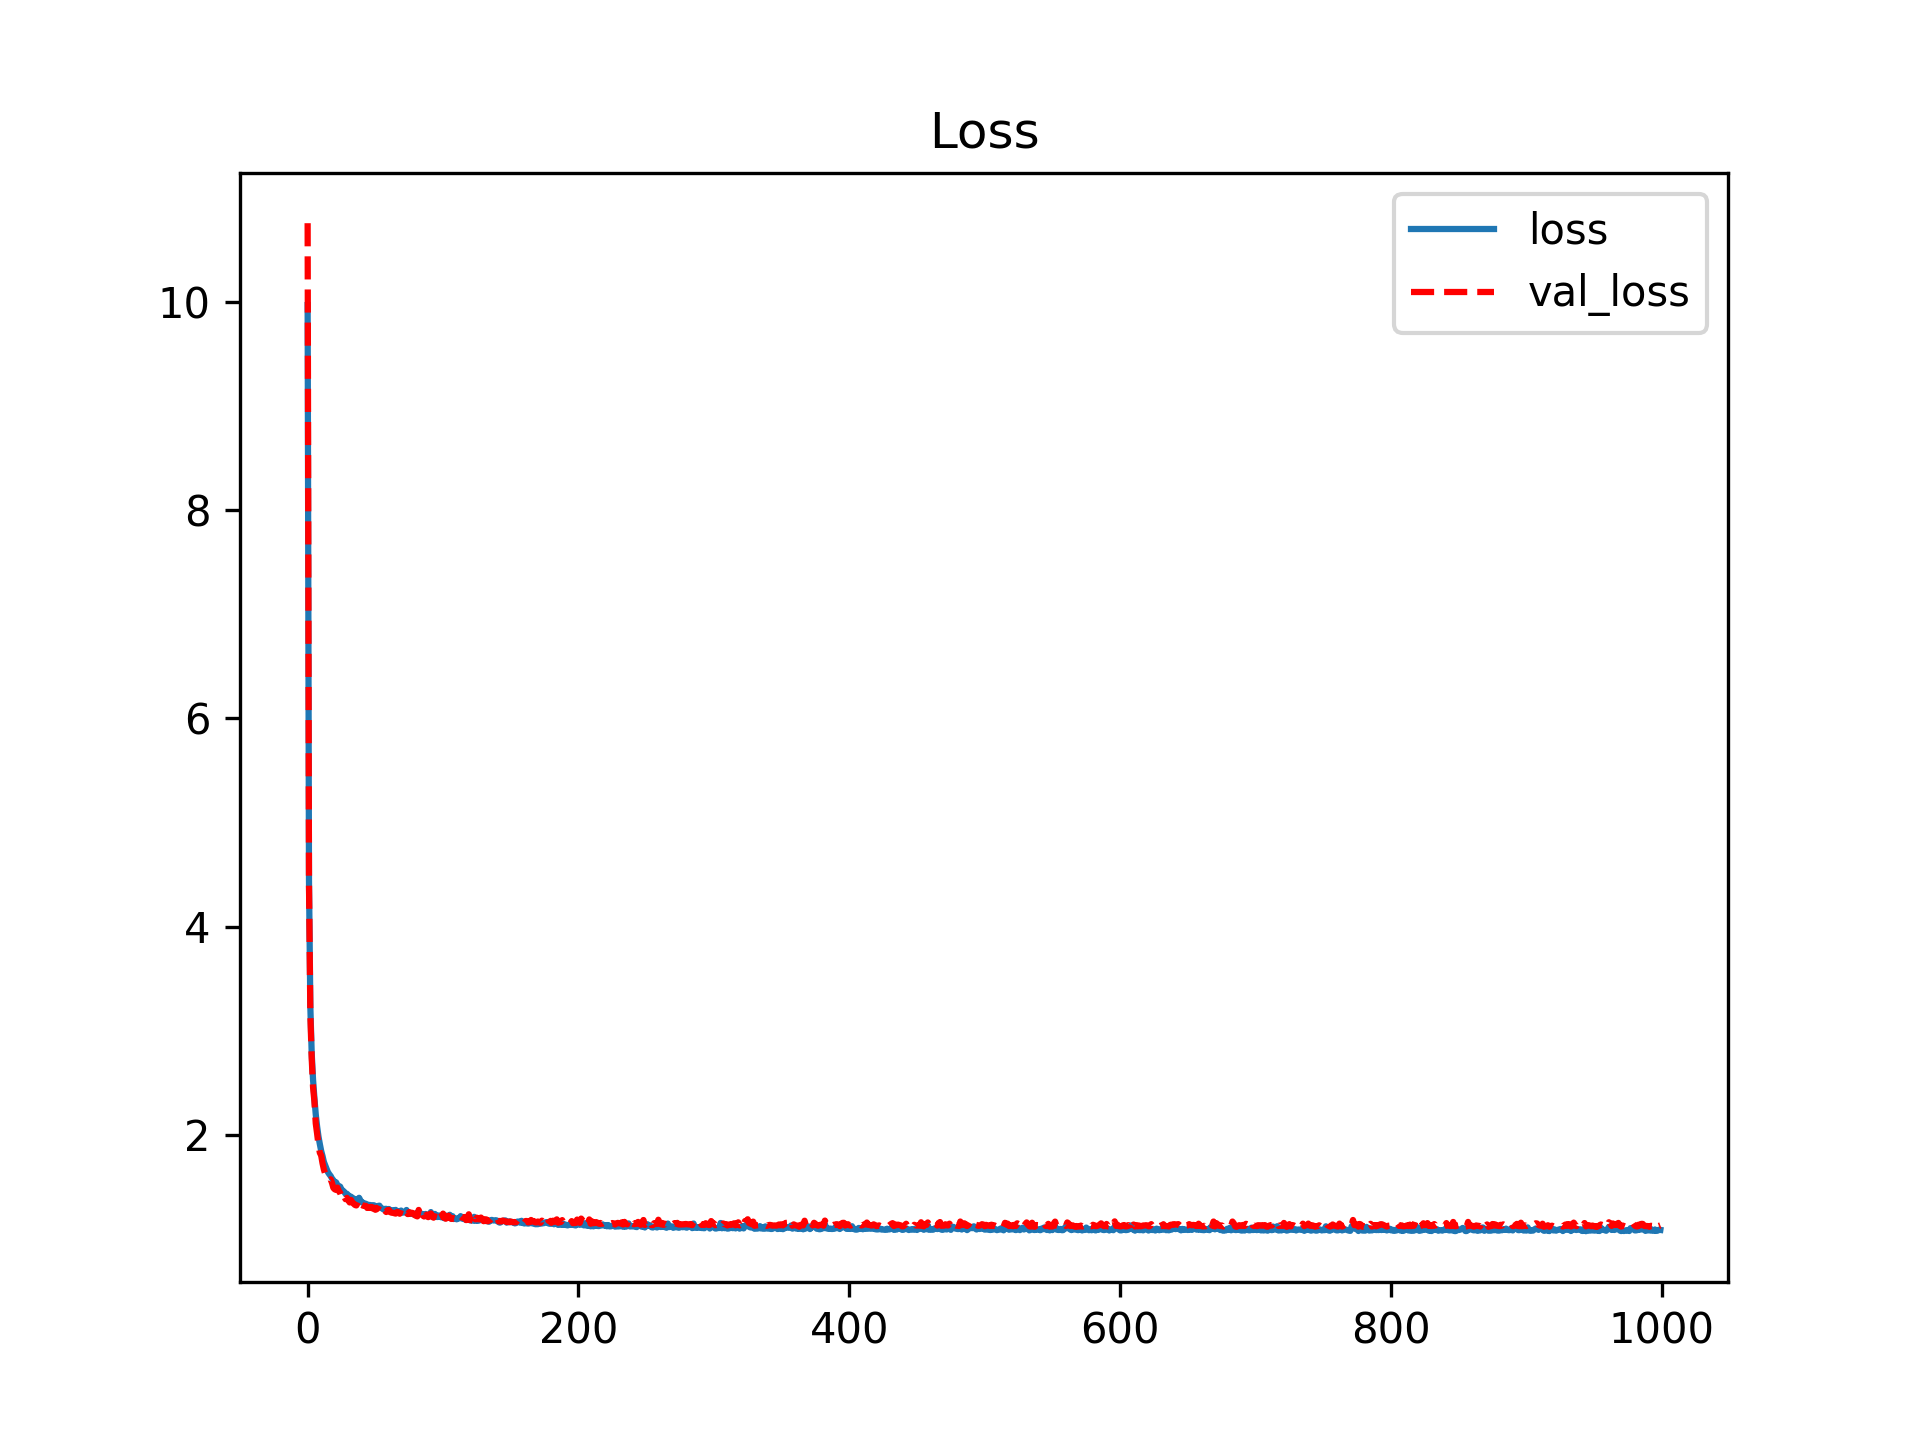
\includegraphics[width=0.55\textwidth]{cup10_one}}
    \subfloat[Type B\label{fig:typeB}]{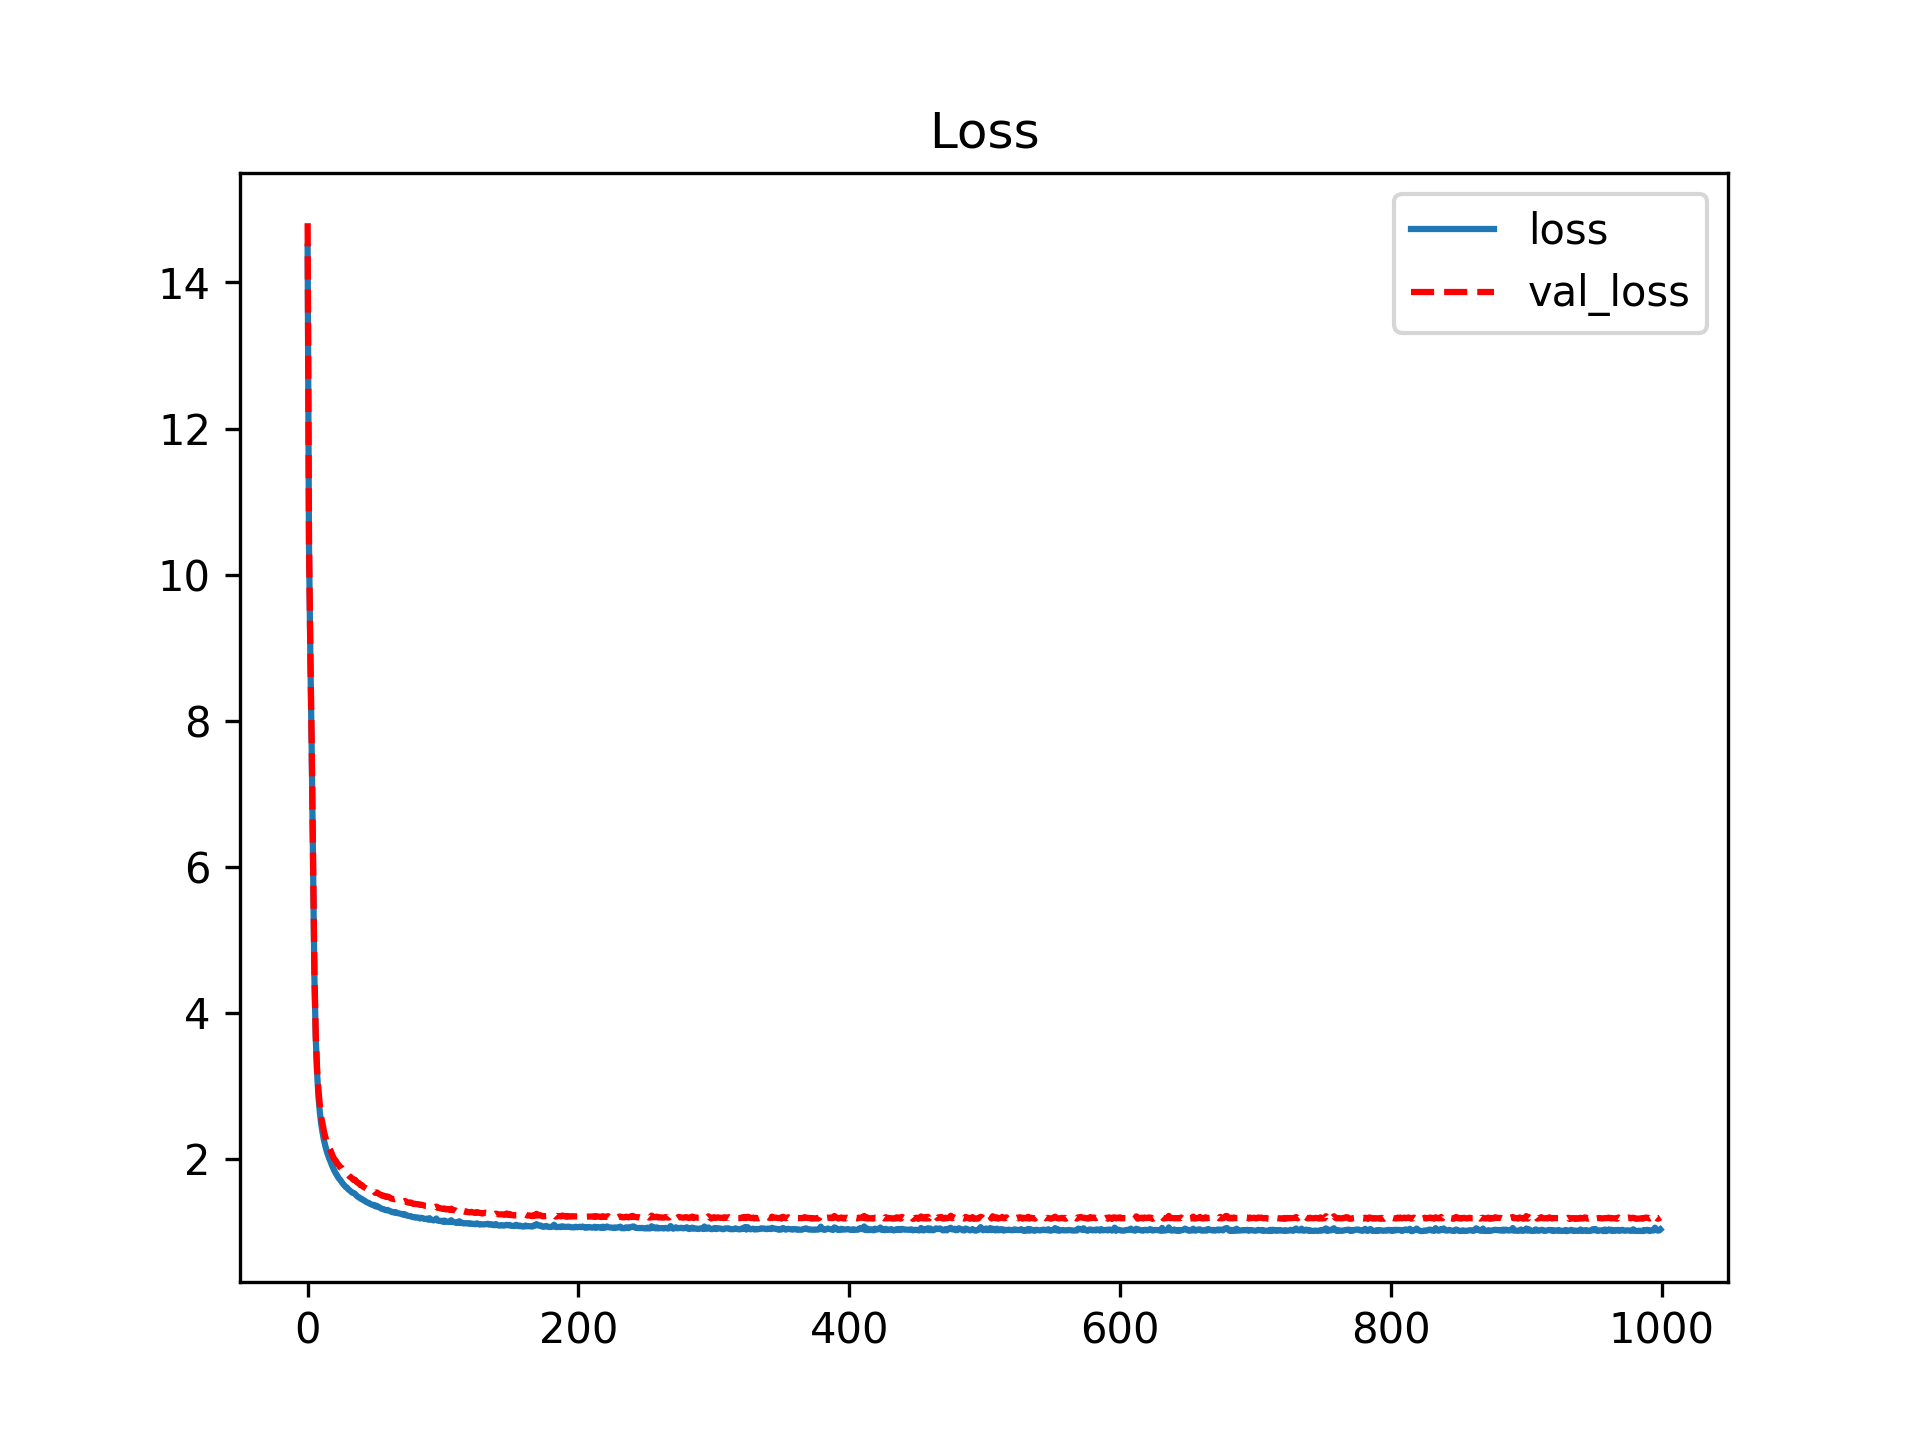
\includegraphics[width=0.55\textwidth]{cup55}}
    \caption{Learning curves for CUP networks}
\end{figure}


Then we tried an \emph{ensemble} approach: we trained 20 networks of type A and regarded the output of our model as the average of the outputs of the 10 bests (over validation benchmark) trained networks.

In this way we achieved a MEE error on the internal test set of $1.085$.

\bigskip
Our last model uses input preprocessing, and we use a different network architecture, say \emph{type B}.
This NN has a topology of 55-20-2, and is trained with $\eta=0.05,\; \lambda=0.005,\; \beta=0.9$.

The 55 inputs are calculated as follows from the dataset: if the original input is $(x_1,\, \dots,\, x_{10})$, our calculated new vector is $(x_1,\, \dots,x_{10},\, x_1\cdot x_2,\, \dots,\, x_9\cdot x_{10})$, that is obtained from the previous one appending the pairwise products of input variables.

Then we took an ensemble approach and trained 20 networks of type B, and we calculate the output by averaging the best 15 of them.

This ensemble of type B models achieved an MEE of $1.050$ on the internal test set.

The learning curve of one instance of model B can be observed in \cref{fig:typeB}. Values of training and validation MEE of some of the 20 models are in \cref{fig:cup55-table} below.

\begin{figure}
    \centering
    \begin{tabular}{|l|l|l|}
        \hline
        id & Train MEE & Valid MEE \\ \hline
        3 & 1.030 & 1.129 \\ \hline
        5 & 0.968 & 1.250 \\ \hline
        8 & 1.038 & 1.081 \\ \hline
        15 & 1.011 & 1.148 \\ \hline
        20 & 0.987 & 1.327 \\ \hline
    \end{tabular}
    \caption{MEE of some elements of a type B networks ensemble}
    \label{fig:cup55-table}
\end{figure}




%%% Local Variables:
%%% mode: latex
%%% TeX-master: "report"
%%% End:
